\section{Mức 5,6 điểm}
\Opensolutionfile{ans}[ans/Muc_5_6]
\setcounter{dang}{0}
\setcounter{ex}{0}
\begin{dang}
	{Thể tích khối lăng trụ đứng}
\end{dang}
\begin{ex}%[2H1Y3-2]%Câu 1.
	(Đề minh họa 2022) Cho khối lăng trụ có diện tích đáy $B$ và chiều cao $h$. Thể tích $V$ của khối lăng trụ đã cho được tính theo công thức nào dưới đây?
	\choice
	{$V=\dfrac{1}{3}Bh$}
	{$V=\dfrac{4}{3}Bh$}
	{$V=6Bh$}
	{\True $V=Bh$}
	\loigiai{
		Định nghĩa thể tích khối lăng trụ là $V=Bh$.}
\end{ex}
\begin{ex}%[2H1Y3-2]%Câu 2.
	(Mã 101-2022) Cho khối lăng trụ có diện tích đáy là $3a^2$ và chiều cao $2a$. Thể tích khối lăng trụ đã cho bằng
	\choice
	{$a^3$}
	{\True $6a^3$}
	{$3a^3$}
	{$2a^3$}
	\loigiai{
		Ta có: $V=B\cdot h=3a^2\cdot 2a=6a^3$.}
\end{ex}
\begin{ex}%[2H1Y3-3]%Câu 3.
	(Mã 104-2022) Cho khối chóp và khối lăng trụ có diện tích đáy, chiều cao tương ứng bằng nhau và có thể tích lần lượt là $V_1,V_2$. Tỉ số $\dfrac{V_1}{V_2}$ bằng
	\choice
	{$\dfrac{2}{3}$}
	{$\dfrac{3}{2}$}
	{$3$}
	{\True $\dfrac{1}{3}$}
	\loigiai{
		Gọi đường cao, diện tích đáy lần lượt là $h,B$.\\
		Khi đó áp dụng công thức thể tích khối chóp, khối lăng trụ ta được $V_1=\dfrac{1}{3}B\cdot h$ và $V_2=B\cdot h$.\\
		Suy ra: $\dfrac{V_1}{V_2}=\dfrac{\dfrac{1}{3}B\cdot h}{B\cdot h}=\dfrac{1}{3}$.}
\end{ex}
\begin{ex}%[2H1Y3-2]%Câu 4.
	(Đề Minh Họa 2021) Thể tích khối hộp chữ nhật có ba kích thước $2, 3, 7$ bằng
	\choice
	{$14$}
	{$42$}
	{$126$}
	{$12$}
	\loigiai{
		Thể tích khối hộp có ba kích thước $2, 3, 7$ bằng $V=abc=2\cdot 3\cdot 7=42$.}
\end{ex}
\begin{ex}%[2H1B3-2]%Câu 5.
	(Mã 101 - 2021 Lần 1) Thể tích của khối lập phương cạnh $5a$ bằng
	\choice
	{$5a^3$}
	{$a^3$}
	{$125a^3$}
	{$25a^3$}
	\loigiai{
		Thể tích của khối lập phương cạnh bằng $5a$ là\\
		$V=(5a)^3=125a^3$.}
\end{ex}
\begin{ex}%[2H1B3-2]%Câu 6.
	(Mã 103 - 2021 - Lần 1) Thể tích khối lập phương có độ dài cạnh $3a$ bằng
	\choice
	{$27a^3$}
	{$3a^3$}
	{$9a^3$}
	{$a^3$}
	\loigiai{
		Thể tích khối lập phương là $(3a)^3=27a^3$.}
\end{ex}
\begin{ex}%[2H1B3-2]%Câu 7.
	(Mã 102 - 2021 Lần 1) Thể tích của khối lập phương cạnh $4a$ bằng
	\choice
	{$64a^3$}
	{$32a^3$}
	{$16a^3$}
	{$8a^3$}
	\loigiai{
		Thể tích của khối lập phương cạnh $4a$ là $V=(4a)^3=64a^3$.}
\end{ex}
\begin{ex}%[2H1B3-2]%Câu 8.
	(Mã 104 - 2021 Lần 1) Thể tích của khối lập phương cạnh $2a$ bằng
	\choice
	{$a^3$}
	{$2a^3$}
	{$8a^3$}
	{$4a^3$}
	\loigiai{
		Ta có $V=(2a)^3=8a^3$.}
\end{ex}
\begin{ex}%[2H1Y3-2]%Câu 9.
	(Mã 101 - 2019) Thể tích khối lăng trụ có diện tích đáy $B$ và có chiều cao $h$ là
	\choice
	{$Bh$}
	{$\dfrac{4}{3}Bh$}
	{$\dfrac{1}{3}Bh$}
	{$3Bh$}
	\loigiai{
		Thể tích khối lăng trụ có diện tích đáy $B$ và có chiều cao $h$ là $V=B\cdot h$.}
\end{ex}
\begin{ex}%[2H1B3-2]%Câu 10.
	(Đề Minh Họa 2020 Lần 1) Cho khối lập phương có cạnh bằng $6$. Thể tích của khối lập phương đã cho bằng
	\choice
	{\True $216$}
	{$18$}
	{$36$}
	{$72$}
	\loigiai{
		Thể tích khối lập phương có cạnh bằng $6$ là $V=6^3=216$.}
\end{ex}
\begin{ex}%[2H1B3-2]%Câu 11.
	(Đề Tham Khảo 2020 Lần 2) Thể tích khối lập phương cạnh $2$ bằng
	\choice
	{$6$}
	{\True $8$}
	{$4$}
	{$2$}
	\loigiai{
		Thể tích khối lập phương cạnh $a$ là $V=a^3$.\\
		Vậy thể tích khối lập phương cạnh $2$ là $V=2^3=8$.}
\end{ex}
\begin{ex}%[2H1B3-2]%Câu 12.
	(Mã 101 - 2020 Lần 1) Cho khối hộp chữ nhật có 3 kích thước $3;4;5$. Thể tích của khối hộp đã cho bằng
	\choice
	{$10$}
	{$20$}
	{$12$}
	{\True $60$}
	\loigiai{
		Thể tích của khối hộp đã cho bằng $V=3\cdot 4\cdot 5=60$.}
\end{ex}
\begin{ex}%[2H1B3-2]%Câu 13.
	(Mã 102 - 2020 Lần 1) Cho khối hộp hình chữ nhật có ba kích thước $2,\,4,\,6$. Thể tích của khối hộp đã cho bằng
	\choice
	{$16$}
	{$12$}
	{\True $48$}
	{$8$}
	\loigiai{
		Thể tích của khối hộp đã cho bằng $2\cdot 4\cdot 6= 48$.}
\end{ex}
\begin{ex}%[2H1B3-2]%Câu 14.
	(Mã 102 - 2020 Lần 2) Cho khối lăng trụ có diện tích đáy $B=3$ và chiều cao $h=2$. Thể tích của khối lăng trụ đã cho bằng
	\choice
	{$1$}
	{$3$}
	{$2$}
	{\True $6$}
	\loigiai{
		Thể tích khối lăng trụ là $V=B\cdot h=3\cdot 2=6$.}
\end{ex}
\begin{ex}%[2H1B3-2]%Câu 15.
	(Mã 103 2018) Cho khối lăng trụ có đáy là hình vuông cạnh $a$ và chiều cao bằng $4a$. Thể tích của khối lăng trụ đã cho bằng
	\choice
	{$16a^3$}
	{$4a^3$}
	{$\dfrac{16}{3}a^3$}
	{$\dfrac{4}{3}a^3$}
	\loigiai{
		$V=S_{day}\cdot h=a^2\cdot 4a=4a^3$.}
\end{ex}
\begin{ex}%[2H1B3-2]%Câu 16.
	(Mã 104 2018) Cho khối lăng trụ có đáy là hình vuông cạnh $a$ và chiều cao bằng $2a$. Thể tích của khối lăng trụ đã cho bằng
	\choice
	{$\dfrac{2}{3}a^3$}
	{$\dfrac{4}{3}a^3$}
	{$2a^3$}
	{$4a^3$}
	\loigiai{
		Ta có: $V_{langtru}=S_{day}\cdot h =a^2\cdot 2a =2a^3$.}
\end{ex}
\begin{ex}%[2H1B3-2]%Câu 17.
	(THPT Thiệu Hóa – Thanh Hóa 2019) Cho khối lăng trụ có diện tích đáy bằng $a^2\sqrt{3}$, khoảng cách giữa hai đáy của lăng trụ bằng $a\sqrt{6}$. Tính thể tích $V$ của khối lăng trụ
	\choice
	{\True $V=3a^3\sqrt{2}$}
	{$V=a^3\sqrt{2}$}
	{$V=\dfrac{a^3\sqrt{2}}{3}$}
	{$V=\dfrac{3a^3\sqrt{2}}{4}$}
	\loigiai{
		Thể tích khối lăng trụ là $V=B\cdot h=a^2\sqrt{3}\cdot a\sqrt{6}=3a^3\sqrt{2}$.}
\end{ex}
%%==========Câu 18
\begin{ex}%[2H1B3-2]	[Mã 102-2019]
	\immini{Cho khối lăng trụ đứng $ABC.A'B'C'$ có đáy là tam giác đều cạnh $a$ và $AA'=2a$ (minh họa như hình vẽ bên).
	Thể tích của khối lăng trụ đã cho bằng
	\choice
	{\True $\dfrac{\sqrt 3a^3}{2}$}
	{$\dfrac{\sqrt 3a^3}{6}$}
	{$\sqrt 3a^3$}
	{$\dfrac{\sqrt 3a^3}{3}$}
}{
	\begin{tikzpicture}
		\def\h{3}
		\def\r{2}
		\def\g{40}
		\path
		(0,0) coordinate (A)
		(0,\h) coordinate(A')
		(-\g:\r) coordinate (B)
		(4,0) coordinate (C)
		($(A')+(B)-(A)$) coordinate (B')
		($(A')+(C)-(A)$) coordinate (C')
		;
		\draw
		(A')--(B')--(C')--cycle
		(A)--(B) (B)--(C)
		(A)--(A') (B)--(B') (C)--(C')			
		;
		\draw[dashed]
		(A)--(C)
		;
		
		\foreach \x/\gm in {A'/90,A/180,B/-90,C/0,B'/90,C'/90}\fill[black](\x) circle (1pt) ($(\x)+(\gm:3mm)$)node{$\x$}
		;
		\def\khgvuong(#1,#2,#3){
			\path
			($(#2)!2mm!(#1)$) coordinate (#2#1)
			($(#2)!2mm!(#3)$) coordinate (#2#3)
			;
			\draw (#2#1)--($(#2#1)+(#2#3)-(#2)$)--(#2#3);
		}
		\khgvuong(A',A,C)
		\khgvuong(A',A,B)
		
		\path ($(A)!0.5!(A')$)node[scale=0.8,above,rotate=90]{$2a$}
		($(A)!0.5!(B)$)node[scale=0.8,below,rotate=-\g]{$a$}
		;
	\end{tikzpicture}
}
\loigiai{
	Tam giác $ABC$ đều cạnh $a$ nên$S_{\Delta ABC}=\dfrac{a^2\sqrt 3}{4}$\\
	Do khối lăng trụ $ABC.A'B'C'$ là lăng trụ đứng nên đường cao của lăng trụ là $AA'=2a$\\
	Thể tích khối lăng trụ là $V=AA'.S_{\Delta ABC}=2a.\dfrac{a^2\sqrt 3}{4}=\dfrac{\sqrt 3a^3}{2}.$
	}
\end{ex}

%%==========Câu 19
\begin{ex}%[2H1K3-2]
	[Đề Minh Họa 2017]
	Tính thể tích $V$ của khối lập phương $ABCD.A'B'C'D'$ , biết $AC'=a\sqrt 3 $.
	\choice
	{\True $V=a^3$}
	{$V=\dfrac{3\sqrt 6a^3}{4}$}
	{$V=3\sqrt 3a^3$}
	{$V=\dfrac{1}{3}{a^3}$}
\loigiai{
	\immini{Giả sử khối lập phương có cạnh bằng $x;\left(x > 0\right)$\\
	Xét tam giác $A'B'C'$ vuông cân tại $B'$ ta có:\\
	$A'C{'^2}=A'B{'^2}+B'C{'^2}$ $=x^2+x^2=2x^2$ $\Rightarrow A'C'=x\sqrt 2 $\\
	Xét tam giác $A'AC'$ vuông tại $A'$ ta có\\
	$AC{'^2}=A'{A^2}+A'C{'^2}$ $\Leftrightarrow 3a^2=x^2+2x^2$ $\Leftrightarrow x=a$\\
	Thể tích của khối lập phương $ABCD.A'B'C'D'$ là $V=a^3$.}
{\begin{tikzpicture}
		\def\h{4}
		\def\r{2}
		\def\g{140}
		\path
		(0,0) coordinate (A)
		(0,\h) coordinate(A')
		(-\g:\r) coordinate (B)
		(4,0) coordinate (D)
		
		($(B)+(D)-(A)$) coordinate (C)
		($(C)+(0,\h)$) coordinate (C')
		($(A')+(B)-(A)$) coordinate (B')
		($(A')+(D)-(A)$) coordinate (D')
		;
		\draw
		(A')--(B')--(C')--(D')--cycle
		(A')--(C')
		(B)--(B') (D)--(D') (B)--(C) (C)--(D) (C)--(C')	
		;
		\draw[dashed]
		(A)--(A') (A)--(B) (A)--(D) (A)--(C')
		;
		
		\foreach \x/\gm in {A/180,B/-90,C/-90,D/0,A'/90,B'/90,C'/90,D'/90}\fill[black](\x) circle (1pt) ($(\x)+(\gm:3mm)$)node{$\x$}
		;
		\def\khgvuong(#1,#2,#3){
			\path
			($(#2)!2mm!(#1)$) coordinate (#2#1)
			($(#2)!2mm!(#3)$) coordinate (#2#3)
			;
			\draw (#2#1)--($(#2#1)+(#2#3)-(#2)$)--(#2#3);
		}
		\khgvuong(A',A,D)
		\khgvuong(A',A,B)
		
		\path ($(A)!0.5!(C')$)node[scale=0.8,above,rotate=45]{$a\sqrt{3}$}
		;
\end{tikzpicture}}
}
\end{ex}

%%==========Câu 20
\begin{ex}%[2H1B3-2]
	[SGD Nam Định] Cho khối lăng trụ đứng $ABC.A'B'C'$ có $B'C=3a$ , đáy $ABC$ là tam giác vuông cân tại $B$ và $AC=a\sqrt 2$. Tính thể tích $V$ của khối lăng trụ đứng $ABC.A'B'C'$.
	\choice
	{$V=2a^3$}
	{$V=\sqrt 2a^3$}
	{\True $V=\dfrac{\sqrt 2a^3}{3}$}
	{$V=\dfrac{a^3}{6\sqrt 2}$}
	\loigiai{
	\immini{Đáy $ABC$ là tam giác vuông cân tại $B$ và $AC=a\sqrt 2\Rightarrow BC=AC=\dfrac{AC}{\sqrt 2}=\dfrac{a\sqrt 2}{\sqrt 2}=a$ .\\
	$\Delta BB'C$ vuông tại $B\Rightarrow BB'=\sqrt{B'C^2-BC^2}=\sqrt{9a^2-a^2}=2a\sqrt 2 $ .\\
	$V=\dfrac{1}{3}\cdot BB'\cdot{S_{\Delta ABC}}=\dfrac{1}{3}2a\sqrt 2\cdot\dfrac{1}{2}\cdot{a^2}=\dfrac{\sqrt 2a^3}{3}$ .\\
	Vậy thể tích của khối lăng trụ đứng $ABC.A'B'C'$ là $V=\dfrac{\sqrt 2a^3}{3}$.}{
	\begin{tikzpicture}
		\def\h{3}
		\def\r{2}
		\def\g{40}
		\path
		(0,0) coordinate (A)
		(0,\h) coordinate(A')
		(-\g:\r) coordinate (B)
		(4,0) coordinate (C)
		($(A')+(B)-(A)$) coordinate (B')
		($(A')+(C)-(A)$) coordinate (C')
		;
		\draw
		(A')--(B')--(C')--cycle
		(A)--(B) (B)--(C)
		(A)--(A') (B)--(B') (C)--(C') (B')--(C)
		;
		\draw[dashed]
		(A)--(C)
		;
		
		\foreach \x/\gm in {A'/90,A/180,B/-90,C/0,B'/90,C'/90}\fill[black](\x) circle (1pt) ($(\x)+(\gm:3mm)$)node{$\x$}
		;
		\def\khgvuong(#1,#2,#3){
			\path
			($(#2)!2mm!(#1)$) coordinate (#2#1)
			($(#2)!2mm!(#3)$) coordinate (#2#3)
			;
			\draw (#2#1)--($(#2#1)+(#2#3)-(#2)$)--(#2#3);
		}
		\khgvuong(A',A,C)
		\khgvuong(A',A,B)
		\khgvuong(A,B,C)
		
		\path ($(B')!0.5!(C)$)node[scale=0.8,above,rotate=-45]{$3a$}
		($(A)!0.5!(C)$)node[scale=0.8,above,rotate=0]{$a\sqrt{2}$}
		;
	\end{tikzpicture}}
}
\end{ex}

%%==========Câu 21
\begin{ex}%[2H1B3-2]
	Cho hình lăng trụ đứng $ABC.A'B'C'$ có đáy $ABC$ là tam giác vuông tại $A$ , biết $AB=a$ , $AC=2a$ và $A'B=3a$ . Tính thể tích của khối lăng trụ $ABC.A'B'C'$ .
	\choice
	{$\dfrac{2\sqrt 2a^3}{3}$}
	{$\dfrac{\sqrt 5a^3}{3}$}
	{$\sqrt 5a^3$}
	{\True $2\sqrt 2a^3$}
	\loigiai{
	\immini{	+ Diện tích đáy là $S_{ABC}=\dfrac{1}{2}AB.AC$ $=\dfrac{1}{2}.a.2a$ $=a^2$ .\\
		+ Tam giác $ABA'$ vuông tại $A$ nên có $AA'=\sqrt{A'{B^2}-A{B^2}}$ $=\sqrt{\left(3a\right)^2-a^2}$ $=2a\sqrt 2 $ .\\
		+ Thể tích cần tính là: $V=S_{ABC}.AA'$ $=a^2.2a\sqrt 2 $ $=2\sqrt 2a^3$.}{
		\begin{tikzpicture}
			\def\h{3}
			\def\r{2}
			\def\g{40}
			\path
			(0,0) coordinate (A)
			(0,\h) coordinate(A')
			(-\g:\r) coordinate (B)
			(4,0) coordinate (C)
			($(A')+(B)-(A)$) coordinate (B')
			($(A')+(C)-(A)$) coordinate (C')
			;
			\draw
			(A')--(B')--(C')--cycle
			(A)--(B) (B)--(C)
			(A)--(A') (B)--(B') (C)--(C') (A')--(B)
			;
			\draw[dashed]
			(A)--(C)
			;
			
			\foreach \x/\gm in {A'/90,A/180,B/-90,C/0,B'/90,C'/90}\fill[black](\x) circle (1pt) ($(\x)+(\gm:3mm)$)node{$\x$}
			;
			\def\khgvuong(#1,#2,#3){
				\path
				($(#2)!2mm!(#1)$) coordinate (#2#1)
				($(#2)!2mm!(#3)$) coordinate (#2#3)
				;
				\draw (#2#1)--($(#2#1)+(#2#3)-(#2)$)--(#2#3);
			}
			\khgvuong(A',A,C)
			\khgvuong(A',A,B)
			\khgvuong(B,A,C)
			
			\path ($(A')!0.5!(B)$)node[scale=0.8,above,rotate=-45]{$3a$}
			($(A)!0.5!(C)$)node[scale=0.8,above,rotate=0]{$2a$}
			($(A)!0.5!(B)$)node[scale=0.8,above,rotate=0]{$a$}
			;
	\end{tikzpicture}}
	}
\end{ex}

%%==========Câu 22
\begin{ex}%[2H1B3-2]
	[Gia Lai 2019] 
	\immini{Cho hình lăng trụ đứng $ABCD.A'B'C'D'$ có đáy $ABCD$ là hình chữ nhật, $AB=a$ , $AD=a\sqrt 2 $ , $AB'=a\sqrt 5 $ (tham khảo hình vẽ). Tính theo $a$ thể tích $V$ của khối lăng trụ đã cho.
	\choice
	{$V=a^3\sqrt 2 $}
	{\True $V=2a^3\sqrt 2 $}
	{$V=a^3\sqrt{10}$}
	{$V=\dfrac{2a^3\sqrt 2}{3}$}
	}{\begin{tikzpicture}
			\def\h{4}
			\def\r{2}
			\def\g{140}
			\path
			(0,0) coordinate (A)
			(0,\h) coordinate(A')
			(-\g:\r) coordinate (B)
			(4,0) coordinate (D)
			
			($(B)+(D)-(A)$) coordinate (C)
			($(C)+(0,\h)$) coordinate (C')
			($(A')+(B)-(A)$) coordinate (B')
			($(A')+(D)-(A)$) coordinate (D')
			;
			\draw
			(A')--(B')--(C')--(D')--cycle
			(B')--(D')
			(B)--(B') (D)--(D') (B)--(C) (C)--(D) (C)--(C')	
			;
			\draw[dashed]
			(A)--(A') (A)--(B) (A)--(D) (A)--(B')
			;
			
			\foreach \x/\gm in {A/180,B/-90,C/-90,D/0,A'/90,B'/90,C'/90,D'/90}\fill[black](\x) circle (1pt) ($(\x)+(\gm:3mm)$)node{$\x$}
			;
			\def\khgvuong(#1,#2,#3){
				\path
				($(#2)!2mm!(#1)$) coordinate (#2#1)
				($(#2)!2mm!(#3)$) coordinate (#2#3)
				;
				\draw (#2#1)--($(#2#1)+(#2#3)-(#2)$)--(#2#3);
			}
			\khgvuong(A',A,D)
			\khgvuong(A',A,B)
			
			\path ($(A)!0.5!(B)$)node[scale=0.8,above,rotate=45]{$a$}
			($(A)!0.5!(D)$)node[scale=0.8,above,rotate=0]{$a\sqrt{2}$}
			($(A)!0.5!(B')$)node[scale=0.8,above,rotate=-45]{$a\sqrt{5}$}
			;
	\end{tikzpicture}}
	\loigiai{
		$S_{ABCD}=AB.AD=a.a\sqrt 2=a^2\sqrt 2 $ .\\
		Trong tam giác $ABB'$ , $BB'=\sqrt{A{B'^2}-A{B^2}}=\sqrt{\left(a\sqrt 5\right)^2-a^2}=2a$ .\\
		Vậy $V=BB'.S_{ABCD}=2a.a^2\sqrt 2=2a^3\sqrt 2 $ .}
\end{ex}

%%==========Câu 23
\begin{ex}%[2H1B3-2]
	Lăng trụ tam giác đều có độ dài tất cả các cạnh bằng 3. Thể tích khối lăng trụ đã cho bằng:
	\choice
	{\True $\dfrac{27\sqrt 3}{4}$}
	{$\dfrac{9\sqrt 3}{2}$}
	{$\dfrac{9\sqrt 3}{4}$}
	{$\dfrac{27\sqrt 3}{2}.$}
	\loigiai{
		Đáy hình lăng trụ là tam giác đều cạnh bằng $3$ nên $S=\dfrac{3^2\sqrt 3}{4}=\dfrac{9\sqrt 3}{4}.$\\
		Chiều cao của hình lăng trụ bằng $h=3$\\
		Thể tích $V=S.h=\dfrac{9\sqrt 3}{4}.3=\dfrac{27\sqrt 3}{4}$ .}
\end{ex}

%%==========Câu 24
\begin{ex}%[2H1Y3-2]
	[Đề Tham Khảo 2019]
	Thể tích của khối lập phương cạnh $2a$ bằng
	\choice
	{\True $8a^3$}
	{$2a^3$}
	{$a^3$}
	{$6a^3$}
	\loigiai{
		Thể tích của khối lập phương cạnh $2a$ bằng: $V=\left(2a\right)^3=8a^3$}
\end{ex}

%%==========Câu 25
\begin{ex}%[2H1B3-2]%
	[Mã 104-2019]
	\immini{Cho khối lăng trụ đứng $ABC.A'B'C'$ có đáy là tam giác đều cạnh $a$ và $AA'=\sqrt 2 a$ (minh họa như hình vẽ bên dưới). Thể tích của khối lăng trụ đã cho bằng
	\choice
	{$\dfrac{\sqrt 6a^3}{2}$}
	{\True $\dfrac{\sqrt 6a^3}{4}$}
	{$\dfrac{\sqrt 6a^3}{6}$}
	{$\dfrac{\sqrt 6a^3}{12}$}
}{
\begin{tikzpicture}
	\def\h{3}
	\def\r{2}
	\def\g{40}
	\path
	(0,0) coordinate (A)
	(0,\h) coordinate(A')
	(-\g:\r) coordinate (B)
	(4,0) coordinate (C)
	($(A')+(B)-(A)$) coordinate (B')
	($(A')+(C)-(A)$) coordinate (C')
	;
	\draw
	(A')--(B')--(C')--cycle
	(A)--(B) (B)--(C)
	(A)--(A') (B)--(B') (C)--(C')			
	;
	\draw[dashed]
	(A)--(C)
	;
	
	\foreach \x/\gm in {A'/90,A/180,B/-90,C/0,B'/90,C'/90}\fill[black](\x) circle (1pt) ($(\x)+(\gm:3mm)$)node{$\x$}
	;
	\def\khgvuong(#1,#2,#3){
		\path
		($(#2)!2mm!(#1)$) coordinate (#2#1)
		($(#2)!2mm!(#3)$) coordinate (#2#3)
		;
		\draw (#2#1)--($(#2#1)+(#2#3)-(#2)$)--(#2#3);
	}
	\khgvuong(A',A,C)
	\khgvuong(A',A,B)
	
	\path ($(A)!0.5!(A')$)node[scale=0.8,above,rotate=90]{$a\sqrt{2}$}
	;
\end{tikzpicture}
}
	\loigiai{
		Ta có: $S_{\Delta ABC}=\dfrac{a^2\sqrt 3}{4}$ .\\
		Vậy thể tích của khối lăng trụ đã cho là\\
		$V_{ABC.A'B'C'}=S_{\Delta ABC}.AA'=\dfrac{a^2\sqrt 3}{4}.a\sqrt 2=\dfrac{a^3\sqrt 6}{4}$ .}
\end{ex}

%%==========Câu 26
\begin{ex}%[2H1B3-2]%
	[Đề Tham Khảo 2017] 
	Thể tích của khối lăng trụ tam giác đều có tất cả các cạnh bằng $a$ .
	\choice
	{$V=\dfrac{a^3\sqrt 3}{12}$}
	{$V=\dfrac{a^3\sqrt 3}{2}$}
	{\True $V=\dfrac{a^3\sqrt 3}{4}$}
	{$V=\dfrac{a^3\sqrt 3}{6}$}
	\loigiai{
		$\left\{\begin{array}{l}
			h=a\\
			S=\dfrac{a^2\sqrt 3}{4}
		\end{array}\right.\Rightarrow V=h.S=\dfrac{a^3\sqrt 3}{4}$}
\end{ex}

%%==========Câu 27
\begin{ex}%[2H1B3-2]%
	[Mã 110-2017] 
	\immini{Cho khối lăng trụ đứng $ABC.A'B'C'$ có $BB'=a$ , đáy $ABC$ là tam giác vuông cân tại $B$ và $AC=a\sqrt 2 $ . Tính thể tích $V$ của khối lăng trụ đã cho.
	\choice
	{$V=\dfrac{a^3}{3}$}
	{\True $V=\dfrac{a^3}{2}$}
	{$V=a^3$}
	{$V=\dfrac{a^3}{6}$}
}{
\begin{tikzpicture}
	\def\h{3}
	\def\r{2}
	\def\g{40}
	\path
	(0,0) coordinate (A)
	(0,\h) coordinate(A')
	(-\g:\r) coordinate (B)
	(4,0) coordinate (C)
	($(A')+(B)-(A)$) coordinate (B')
	($(A')+(C)-(A)$) coordinate (C')
	;
	\draw
	(A')--(B')--(C')--cycle
	(A)--(B) (B)--(C)
	(A)--(A') (B)--(B') (C)--(C')
	;
	\draw[dashed]
	(A)--(C)
	;
	
	\foreach \x/\gm in {A'/90,A/180,B/-90,C/0,B'/90,C'/90}\fill[black](\x) circle (1pt) ($(\x)+(\gm:3mm)$)node{$\x$}
	;
	\def\khgvuong(#1,#2,#3){
		\path
		($(#2)!2mm!(#1)$) coordinate (#2#1)
		($(#2)!2mm!(#3)$) coordinate (#2#3)
		;
		\draw (#2#1)--($(#2#1)+(#2#3)-(#2)$)--(#2#3);
	}
	\khgvuong(A',A,C)
	\khgvuong(A',A,B)
	\khgvuong(A,B,C)
	
	\path ($(A)!0.5!(A')$)node[scale=0.8,above,rotate=90]{$a$}
	($(A)!0.5!(C)$)node[scale=0.8,above,rotate=0]{$a\sqrt{2}$}
	;
\end{tikzpicture}}
	\loigiai{
		Tam giác $ABC$ vuông cân tại $B$ $\Rightarrow AB=BC=\dfrac{AC}{\sqrt 2}=a$ . Suy ra: $S_{ABC}=\dfrac{1}{2}{a^2}$ .\\
		Khi đó: $V_{ABC.A'B'C'}=S_{ABC}.BB'=\dfrac{1}{2}{a^2}.a=\dfrac{a^3}{2}$}
\end{ex}

%%==========Câu 28
\begin{ex}%[2H1B3-2]%
	[Mã 103-2019] 
	\immini{Cho khối lăng trụ đứng $ABC.A'B'C'$ có đáy là tam giác đều cạnh $2a$ và $AA'=3a$ (minh họa như hình vẽ bên). Thể tích của khối lăng trụ đã cho bằng
	\choice
	{$6\sqrt 3a^3$}
	{\True $3\sqrt 3a^3$}
	{$2\sqrt 3a^3$}
	{$\sqrt 3a^3$}
}{
\begin{tikzpicture}
	\def\h{3}
	\def\r{2}
	\def\g{40}
	\path
	(0,0) coordinate (A)
	(0,\h) coordinate(A')
	(-\g:\r) coordinate (B)
	(4,0) coordinate (C)
	($(A')+(B)-(A)$) coordinate (B')
	($(A')+(C)-(A)$) coordinate (C')
	;
	\draw
	(A')--(B')--(C')--cycle
	(A)--(B) (B)--(C)
	(A)--(A') (B)--(B') (C)--(C')
	;
	\draw[dashed]
	(A)--(C)
	;
	
	\foreach \x/\gm in {A'/90,A/180,B/-90,C/0,B'/90,C'/90}\fill[black](\x) circle (1pt) ($(\x)+(\gm:3mm)$)node{$\x$}
	;
	\def\khgvuong(#1,#2,#3){
		\path
		($(#2)!2mm!(#1)$) coordinate (#2#1)
		($(#2)!2mm!(#3)$) coordinate (#2#3)
		;
		\draw (#2#1)--($(#2#1)+(#2#3)-(#2)$)--(#2#3);
	}
	\khgvuong(A',A,C)
	\khgvuong(A',A,B)
	
	\path ($(A)!0.5!(A')$)node[scale=0.8,above,rotate=90]{$3a$}
	($(A)!0.5!(C)$)node[scale=0.8,above,rotate=0]{$a$}
	;
\end{tikzpicture}}
	\loigiai{
		Khối lăng trụ đã cho có đáy là tam giác đều có diện tích là $\dfrac{(2a)^2\sqrt 3}{4}$ và chiều cao là $AA'=3a$ (do là lăng trụ đứng) nên có thể tích là $\dfrac{(2a)^2\sqrt 3}{4}.3a=3\sqrt 3a^3$}
\end{ex}

%%==========Câu 29
\begin{ex}%[2H1B3-2]%
	[Mã 101-2019] 
	\immini{Cho khối lăng trụ đứng $ABC.A'B'C'$ có đáy là tam giác đều
	cạnh $a$ và $AA'=\sqrt 3 a$ (minh họa hình vẽ bên). Thể tích khối lăng trụ đã cho bằng.
	\choice
	{$\dfrac{a^3}{4}$}
	{$\dfrac{a^3}{2}$}
	{\True $\dfrac{3a^3}{4}$}
	{$\dfrac{3a^3}{2}$}
}{
\begin{tikzpicture}
	\def\h{3}
	\def\r{2}
	\def\g{40}
	\path
	(0,0) coordinate (A)
	(0,\h) coordinate(A')
	(-\g:\r) coordinate (B)
	(4,0) coordinate (C)
	($(A')+(B)-(A)$) coordinate (B')
	($(A')+(C)-(A)$) coordinate (C')
	;
	\draw
	(A')--(B')--(C')--cycle
	(A)--(B) (B)--(C)
	(A)--(A') (B)--(B') (C)--(C')
	;
	\draw[dashed]
	(A)--(C)
	;
	
	\foreach \x/\gm in {A'/90,A/180,B/-90,C/0,B'/90,C'/90}\fill[black](\x) circle (1pt) ($(\x)+(\gm:3mm)$)node{$\x$}
	;
	\def\khgvuong(#1,#2,#3){
		\path
		($(#2)!2mm!(#1)$) coordinate (#2#1)
		($(#2)!2mm!(#3)$) coordinate (#2#3)
		;
		\draw (#2#1)--($(#2#1)+(#2#3)-(#2)$)--(#2#3);
	}
	\khgvuong(A',A,C)
	\khgvuong(A',A,B)
	
	\path ($(A)!0.5!(A')$)node[scale=0.8,above,rotate=90]{$a\sqrt{3}$}
	($(A)!0.5!(C)$)node[scale=0.8,above,rotate=0]{$a$}
	;
\end{tikzpicture}}
	\loigiai{
		Ta có $S_{ABC}=\dfrac{a^2\sqrt 3}{4}$ ; $AA'=a\sqrt 3 $ . Từ đó suy ra $V=a\sqrt 3 .a^2\dfrac{\sqrt 3}{4}=\dfrac{3a^3}{4}$.}
\end{ex}

%%==========Câu 30
\begin{ex}%[2H1B3-2]%
	[THPT Việt Đức Hà Nội Năm 2019] 
	Cho hình lăng trụ đứng $ABC.A'B'C'$ có đáy là tam giác vuông cân tại $B$ , $AB=a$ và $A'B=a\sqrt 3 $. Thể tích khối lăng trụ $ABC.A'B'C'$ là
	\choice
	{$\dfrac{a^3\sqrt 3}{2}$}
	{$\dfrac{a^3}{6}$}
	{$\dfrac{a^3}{2}$}
	{\True $\dfrac{a^3\sqrt 2}{2}$}
	\loigiai{
	\immini{Ta có $AA'=\sqrt{A'{B^2}-A{B^2}}=a\sqrt 2 $ , $S_{ABC}=\dfrac{1}{2}A{B^2}=\dfrac{a^2}{2}$ .\\
	Thể tích khối lăng trụ là $V=AA'.S_{ABC}=\dfrac{a^3\sqrt 2}{2}$.
}{
\begin{tikzpicture}
	\def\h{3}
	\def\r{2}
	\def\g{40}
	\path
	(0,0) coordinate (A)
	(0,\h) coordinate(A')
	(-\g:\r) coordinate (B)
	(4,0) coordinate (C)
	($(A')+(B)-(A)$) coordinate (B')
	($(A')+(C)-(A)$) coordinate (C')
	;
	\draw
	(A')--(B')--(C')--cycle
	(A)--(B) (B)--(C)
	(A)--(A') (B)--(B') (C)--(C') (A')--(B)
	;
	\draw[dashed]
	(A)--(C)
	;
	
	\foreach \x/\gm in {A'/90,A/180,B/-90,C/0,B'/90,C'/90}\fill[black](\x) circle (1pt) ($(\x)+(\gm:3mm)$)node{$\x$}
	;
	\def\khgvuong(#1,#2,#3){
		\path
		($(#2)!2mm!(#1)$) coordinate (#2#1)
		($(#2)!2mm!(#3)$) coordinate (#2#3)
		;
		\draw (#2#1)--($(#2#1)+(#2#3)-(#2)$)--(#2#3);
	}
	\khgvuong(A',A,C)
	\khgvuong(A',A,B)
	\khgvuong(A,B,C)
	
	\path ($(A)!0.5!(B)$)node[scale=0.8,above,rotate=-\g]{$a$}
	($(A')!0.5!(B)$)node[scale=0.8,above,rotate=-60]{$a\sqrt{3}$}
	;
\end{tikzpicture}}
}
\end{ex}

%%==========Câu 31
\begin{ex}%[2H1B3-2]%
	Cho hình lăng trụ đứng $ABC.A'B'C'$ có đáy là tam giác đều cạnh $a$, $A'B$ tạo với mặt phẳng đáy một góc $60^{\rm{o}}$. Thể tích khối lăng trụ $ABC.A'B'C'$ bằng
	\choice
	{$\dfrac{3a^3}{2}$}
	{$\dfrac{a^3}{4}$}
	{\True $\dfrac{3a^3}{4}$}
	{$\dfrac{3a^3}{8}$}
	\loigiai{
	\immini{Đáy là tam giác đều cạnh $a$, có diện tích: $S_{\Delta ABC}=\dfrac{a^2\sqrt 3}{4}$.\\
	Vì $AA'\perp\left(ABC\right)\Rightarrow\widehat{A'BA}=\left(A'B,\left(ABC\right)\right)=60^{\rm{o}}$ , suy ra: $AA'=AB\tan{60^{\rm{o}}}=a\sqrt 3 $\\
	Vậy thể tích khối lăng trụ:\\
		$V_{ABC.A'B'C'}=S_{\Delta ABC}.AA'=\dfrac{a^2\sqrt 3}{4}.a\sqrt 3=\dfrac{3a^3}{4}.$
	}{
	\begin{tikzpicture}
		\def\h{3}
		\def\r{2}
		\def\g{40}
		\path
		(0,0) coordinate (A)
		(0,\h) coordinate(A')
		(-\g:\r) coordinate (B)
		(4,0) coordinate (C)
		($(A')+(B)-(A)$) coordinate (B')
		($(A')+(C)-(A)$) coordinate (C')
		;
		\draw
		(A')--(B')--(C')--cycle
		(A)--(B) (B)--(C)
		(A)--(A') (B)--(B') (C)--(C') (A')--(B)
		;
		\draw[dashed]
		(A)--(C)
		;
		
		\foreach \x/\gm in {A'/90,A/180,B/-90,C/0,B'/90,C'/90}\fill[black](\x) circle (1pt) ($(\x)+(\gm:3mm)$)node{$\x$}
		;
		\def\khgvuong(#1,#2,#3){
			\path
			($(#2)!2mm!(#1)$) coordinate (#2#1)
			($(#2)!2mm!(#3)$) coordinate (#2#3)
			;
			\draw (#2#1)--($(#2#1)+(#2#3)-(#2)$)--(#2#3);
		}
		\khgvuong(A',A,C)
		\khgvuong(A',A,B)
		\khgvuong(A,B,C)
		
		\path ($(A)!0.5!(B)$)node[scale=0.8,above,rotate=0]{$60^\circ$}
		;
\end{tikzpicture}}
}
\end{ex}

%%==========Câu 32
\begin{ex}%[2H1K3-2]%
	Cho hình lăng trụ đứng $ABCD.A'B'C'D'$, đáy là hình thang vuông tại $A$ và $D$, có $AB=2CD,AD=CD=a\sqrt 2 ,AA'=2a$. Thể tích khối lăng trụ đã cho bằng
	\choice
	{$12a^3$}
	{\True $6a^3$}
	{$2a^3$}
	{$4a^3$}
	\loigiai{
	\immini{Diện tích hình thang $ABCD$ là:\\
		$S_{ABCD}$ $=\dfrac{\left(AB+CD\right).AD}{2}$ $=\dfrac{\left(2CD+CD\right).AD}{2}$ $=\dfrac{3CD.AD}{2}$ $=\dfrac{3.a\sqrt 2 .a\sqrt 2}{2}$ $=3a^2$ .\\
		Thể tích khối lăng trụ đã cho: $V=S_{ABCD}.AA'$ $=3a^2.2a$ $=6a^3$.
	}{
	\begin{tikzpicture}
		\def\h{3}
		\def\r{2}
		\def\g{40}
		\path
		(0,0) coordinate (A)
		(0,\h) coordinate(A')
		(4,0) coordinate (B)
		(1,-1) coordinate (C)
		(-1,-1) coordinate (D)
		($(A')+(B)-(A)$) coordinate (B')
		($(A')+(C)-(A)$) coordinate (C')
		($(D)+(0,\h)$) coordinate (D')
		;
		\draw
		(A')--(B')--(C')--(D')--cycle
		(B)--(C)--(D)--(D')
		(B)--(B') (C)--(C')
		;
		\draw[dashed]
		(A')--(A)--(B) (A)--(D)
		;
		
		\foreach \x/\gm in {A'/90,A/45,B/-90,C/-90,D/180,B'/90,C'/90,D'/180}\fill[black](\x) circle (1pt) ($(\x)+(\gm:3mm)$)node{$\x$}
		;
		\def\khgvuong(#1,#2,#3){
			\path
			($(#2)!2mm!(#1)$) coordinate (#2#1)
			($(#2)!2mm!(#3)$) coordinate (#2#3)
			;
			\draw (#2#1)--($(#2#1)+(#2#3)-(#2)$)--(#2#3);
		}
		\khgvuong(D,A,B)
		\khgvuong(A,D,C)
				
		\path ($(A)!0.5!(D)$)node[scale=0.8,above,rotate=50]{$a\sqrt{2}$}
		($(A)!0.5!(A')$)node[scale=0.8,above,rotate=90]{$2a$}
		($(C)!0.5!(D)$)node[scale=0.8,above,rotate=0]{$a\sqrt{2}$}
		;
\end{tikzpicture}}
}
\end{ex}

%%==========Câu 33
\begin{ex}%[2H1B3-2]%
	[Chuyên Lê Quý Đôn Điện Biên 2019] 
	Tính thể tích khối lăng trụ đứng $ABC.A'B'C'$ biết $AA'=2a;AB=3a;AC=4a$ và $AB\perp AC$ .
	\choice
	{\True $12a^3$}
	{$4a^3$}
	{$24a^3$}
	{$8a^3$}
	\loigiai{
	\immini{	Ta có:$S_{ABC}=\dfrac{1}{2}AB.AC=\dfrac{1}{2}3a.4a=6a^2$ .\\
		Vậy $V_{ABC.A'B'C'}=AA'.S_{ABC}=12a^3$.
	}{
	\begin{tikzpicture}
		\def\h{3}
		\def\r{2}
		\def\g{40}
		\path
		(0,0) coordinate (A)
		(0,\h) coordinate(A')
		(-\g:\r) coordinate (B)
		(4,0) coordinate (C)
		($(A')+(B)-(A)$) coordinate (B')
		($(A')+(C)-(A)$) coordinate (C')
		;
		\draw
		(A')--(B')--(C')--cycle
		(A)--(B) (B)--(C)
		(A)--(A') (B)--(B') (C)--(C')
		;
		\draw[dashed]
		(A)--(C)
		;
		
		\foreach \x/\gm in {A'/90,A/180,B/-90,C/0,B'/90,C'/90}\fill[black](\x) circle (1pt) ($(\x)+(\gm:3mm)$)node{$\x$}
		;
		\def\khgvuong(#1,#2,#3){
			\path
			($(#2)!2mm!(#1)$) coordinate (#2#1)
			($(#2)!2mm!(#3)$) coordinate (#2#3)
			;
			\draw (#2#1)--($(#2#1)+(#2#3)-(#2)$)--(#2#3);
		}
		\khgvuong(A',A,C)
		\khgvuong(A',A,B)
		\khgvuong(B,A,C)
		
		\path ($(A)!0.5!(B)$)node[scale=0.8,above,rotate=0]{$3a$}
		($(A)!0.5!(C)$)node[scale=0.8,above,rotate=0]{$4a$}
		($(A)!0.5!(A')$)node[scale=0.8,above,rotate=90]{$2a$}
		;
\end{tikzpicture}}
}
\end{ex}

%%==========Câu 34
\begin{ex}%[2H1B3-2]%
	[Hội 8 trường chuyên ĐBSH-2019] Cho hình lăng trụ đứng $ABCD.A'B'C'D'$ có đáy là hình thoi, biết $AA'=4a,\;AC=2a,\;BD=a$. Thể tích $V$ của khối lăng trụ là
	\choice
	{$V=8a^3$}
	{$V=2a^3$}
	{$V=\dfrac{8}{3}{a^3}$}
	{\True $V=4a^3$}
	\loigiai{
	\immini{	Thể tích $V$ của khối lăng trụ là: $V=S_{ABCD}.AA'=\dfrac{1}{2}.AC.BD.AA'=\dfrac{1}{2}.2a.a.4a=4a^3$.
	}{\begin{tikzpicture}
		\def\h{3}
		\def\r{2}
		\def\g{140}
		\path
		(0,0) coordinate (A)
		(0,\h) coordinate(A')
		(-\g:\r) coordinate (B)
		(4,0) coordinate (D)
		
		($(B)+(D)-(A)$) coordinate (C)
		($(C)+(0,\h)$) coordinate (C')
		($(A')+(B)-(A)$) coordinate (B')
		($(A')+(D)-(A)$) coordinate (D')
		($(A)!0.5!(C)$) coordinate (I)
		;
		\draw
		(A')--(B')--(C')--(D')--cycle
		(B)--(B') (D)--(D') (B)--(C) (C)--(D) (C)--(C')	
		;
		\draw[dashed]
		(A)--(A') (A)--(B) (A)--(D) (A)--(C) (B)--(D)
		;
		
		\foreach \x/\gm in {A/180,B/-90,C/-90,D/0,A'/90,B'/90,C'/90,D'/90}\fill[black](\x) circle (1pt) ($(\x)+(\gm:3mm)$)node{$\x$}
		;
		\def\khgvuong(#1,#2,#3){
			\path
			($(#2)!2mm!(#1)$) coordinate (#2#1)
			($(#2)!2mm!(#3)$) coordinate (#2#3)
			;
			\draw (#2#1)--($(#2#1)+(#2#3)-(#2)$)--(#2#3);
		}
		\khgvuong(A',A,D)
		\khgvuong(A',A,B)
		\khgvuong(A,I,D)
		
		\path ($(A)!0.5!(A')$)node[scale=0.8,above,rotate=90]{$4a$}
		;
\end{tikzpicture}}
	}
\end{ex}

%%==========Câu 35
\begin{ex}%[2H1B3-2]%
	[THPT Phan Bội Châu-Nghệ An 2019] Cho hình hộp đứng có một mặt là hình vuông cạnh $a$ và một mặt có diện tích là $3\rm{a}^2$. Thể tích khối hộp là
	\choice
	{$a^3$}
	{\True $3a^3$}
	{$2a^3$}
	{$4\rm{a}^3$}
	\loigiai{
	\immini{	Giả sử mặt $ABB'A'$ là hình vuông cạnh bằng $a$, mặt $ABCD$ có diện tích bằng $3\rm{a}^2$.\\
	Do đó chiều cao $h=AA'=a$, diện tích đáy là $B=S_{ABCD}=3\rm{a}^2$.\\
	Suy ra thể tích của khối hộp đó là $V=3{a}^2a=3{a}^3$.
	}{\begin{tikzpicture}
		\def\h{3}
		\def\r{2}
		\def\g{140}
		\path
		(0,0) coordinate (A)
		(0,\h) coordinate(A')
		(-\g:\r) coordinate (B)
		(4,0) coordinate (D)
		
		($(B)+(D)-(A)$) coordinate (C)
		($(C)+(0,\h)$) coordinate (C')
		($(A')+(B)-(A)$) coordinate (B')
		($(A')+(D)-(A)$) coordinate (D')
		($(A)!0.5!(C)$) coordinate (I)
		;
		\draw
		(A')--(B')--(C')--(D')--cycle
		(B)--(B') (D)--(D') (B)--(C) (C)--(D) (C)--(C')	
		;
		\draw[dashed]
		(A)--(A') (A)--(B) (A)--(D)
		;
		
		\foreach \x/\gm in {A/180,B/-90,C/-90,D/0,A'/90,B'/90,C'/90,D'/90}\fill[black](\x) circle (1pt) ($(\x)+(\gm:3mm)$)node{$\x$}
		;
\end{tikzpicture}}
	}
\end{ex}

%%==========Câu 36
\begin{ex}%[2H1B3-2]%
	[Chuyên Bắc Giang 2019] Cho khối hộp chữ nhật $ABCD.A'B'C'D'$, biết $AB=a\,;\,BC=2a\,;\,AC'=a\sqrt{21}$. Tính thể tích $V$ của khối hộp đó?
	\choice
	{$4a^3$}
	{$16a^3$}
	{$\dfrac{8}{3}{a^3}$}
	{\True $8a^3$}
\loigiai{
	\immini{Xét tam giác vuông $ABC$, ta có: $AC=\sqrt{A{B^2}+B{C^2}}=a\sqrt 5 $.\\
	Xét tam giác vuông $ACC'$, ta có: $CC'=\sqrt{A{C'^2}-A{C^2}}=4a$.\\
	Vậy thể tích của khối hộp hộp chữ nhật $ABCD\,\cdot \,A'B'C'D'$ là: $V=a\,\cdot \,2a\,\cdot\,4a=8a^3$.}{\begin{tikzpicture}
		\def\h{3}
		\def\r{2}
		\def\g{140}
		\path
		(0,0) coordinate (A)
		(0,\h) coordinate(A')
		(-\g:\r) coordinate (B)
		(4,0) coordinate (D)
		
		($(B)+(D)-(A)$) coordinate (C)
		($(C)+(0,\h)$) coordinate (C')
		($(A')+(B)-(A)$) coordinate (B')
		($(A')+(D)-(A)$) coordinate (D')
		;
		\draw
		(A')--(B')--(C')--(D')--cycle
		(B)--(B') (D)--(D') (B)--(C) (C)--(D) (C)--(C')	
		;
		\draw[dashed]
		(A)--(A') (A)--(B) (A)--(D) (A)--(C') (A)--(C)
		;
		
		\foreach \x/\gm in {A/180,B/-90,C/-90,D/0,A'/90,B'/90,C'/90,D'/90}\fill[black](\x) circle (1pt) ($(\x)+(\gm:3mm)$)node{$\x$}
		;
		
		\path ($(A)!0.5!(B)$)node[scale=0.8,above,rotate=0]{$a$}
		($(B)!0.5!(C)$)node[scale=0.8,above,rotate=0]{$2a$}
		($(A)!0.5!(C')$)node[scale=0.8,above,rotate=45]{$a\sqrt{21}$}
		;
\end{tikzpicture}}
}
\end{ex}
%%==========Câu 37
\begin{ex}%[2H1B3-2][THPT Thăng Long 2019]
	Hình lập phương có độ dài đường chéo bằng $6$ thì có thể tích là
	\choice
	{$2\sqrt{2}$}
	{$54\sqrt{2}$}
	{\True $24\sqrt{3}$}
	{$8$}
	\loigiai{
		Gọi cạnh của hình lập phương là $a\left(a>0\right)$. \\
		$\Rightarrow $ đường chéo của hình lập phương là $a\sqrt{3}$. \\
		Theo bài ra ta có $a\sqrt{3}=6\Rightarrow a=2\sqrt{3}$. \\
		Vậy thể tích của khối lập phương là: $V={\left(2\sqrt{3}\right)}^3=24\sqrt{3}$. 
	}
\end{ex}
%%==========Câu 38
\begin{ex}%[2H1B3-2]
	Cho khối hộp chữ nhật $ABCD.A'B'C'D'$ có $AA'=a$, $AB=3a$, $AC=5a$. Thể tích của khối hộp đã cho là
	\choice
	{$5a^3$}
	{$4a^3$}
	{\True $12a^3$}
	{$15a^3$}
	\loigiai{
		\immini{Xét $\Delta ABC$ vuông tại $B$, ta có \break $BC=\sqrt{AC^2-AB^2}=\sqrt{{\left(5a\right)}^2-{\left(3a\right)}^2}=4a$. \\
			$S_{ABCD}=AB\cdot BC=3a\cdot 4a=12a^2$.\\
			$V_{ABCD.A'B'C'D'}=S_{ABCD}\cdot AA'=12a^2\cdot a=12a^3$. }
		{
			\begin{tikzpicture}[scale=1, font=\footnotesize, line join=round, line cap=round, >=stealth]
				\path 
				(0,0) coordinate (A)
				(-2,-1) coordinate (B)
				(4,0) coordinate (D)
				($(B)+(D)-(A)$) coordinate (C)
				;
				\foreach \x in {A,B,C,D} \path (\x)+(0,3) coordinate (\x');
				\draw (A')--(B')--(B)--(C)--(D)--(D')--cycle (B')--(C')--(D') (C)--(C');
				\draw[dashed] (A)--(C) (B)--(A)--(D) (A)--(A');
				
				\foreach \p/\r in {A/180,B/-120,C/-60,D/-60,D'/60,A'/90,B'/180,C'/135}
				\fill (\p) circle (1.5pt) node[shift={(\r:3mm)}]{$\p$};
			\end{tikzpicture}
		}
	}
\end{ex}
%%==========Câu 39
\begin{ex}%[2H1B3-2][HKI-NK HCM-2019]
	Cho hình hộp đứng có cạnh bên độ dài $3a$, đáy là hình thoi cạnh $a$ và có một góc $60^\circ $. Khi đó thể tích khối hộp là
	\choice
	{$\dfrac{3a^3\sqrt{3}}{4}$}
	{$\dfrac{a^3\sqrt{3}}{3}$}
	{$\dfrac{a^3\sqrt{3}}{2}$}
	{\True $\dfrac{3a^3\sqrt{3}}{2}$}
	\loigiai{
		Ta có chiều cao $h=3a$. \\
		Hình thoi cạnh a và có một góc $60^\circ $ có diện tích $S=2. \dfrac{a^2\sqrt{3}}{4}=\dfrac{a^2\sqrt{3}}{2}$.\\
		Thể tích khối hộp là $V=S\cdot h=\dfrac{a^2\sqrt{3}}{2}\cdot3a=\dfrac{3a^3\sqrt{3}}{2}$. 
	}
\end{ex}
%%==========Câu 40
\begin{ex}%[2H1B3-2][Chuyên Lam Sơn 2019]
	Cho hình lăng trụ đứng $ABC.A'B'C'$ có $BB'=a$, đáy $ABC$ là tam giác vuông cân tại $B$, $AC=a\sqrt{2}$. Tính thể tích lăng trụ
	\choice
	{$\dfrac{a^3}{3}$}
	{$\dfrac{a^3}{6}$}
	{$a^3$}
	{\True $\dfrac{a^3}{2}$}
	\loigiai{
		\immini{Trong $\Delta ABC$ có $AC^2=AB^2+BC^2\\
			\Leftrightarrow 2AB^2={\left(a\sqrt{2}\right)}^2\Leftrightarrow AB=BC=a $.\\
			Thể tích khối lăng trụ $ABC.A'B'C'$ là\\ $V_{ABC.A'B'C'}=S_{\Delta ABC}\cdot BB'\\
			=\dfrac{1}{2}AB\cdot BC\cdot BB'=\dfrac{1}{2}\cdot a\cdot a \cdot a=\dfrac{a^3}{2} $.}
		{
			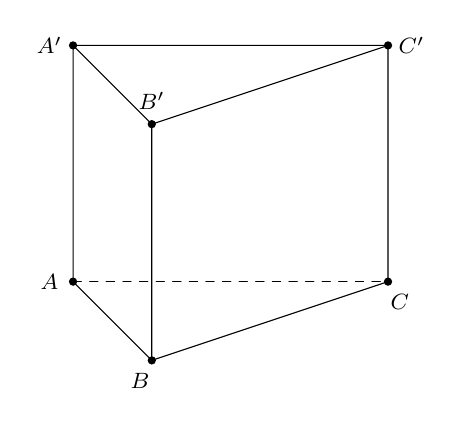
\begin{tikzpicture}[scale=1, font=\footnotesize, line join=round, line cap=round, >=stealth]
				\path 
				(0,0) coordinate (A)
				(1,-1) coordinate (B)
				(4,0) coordinate (C)
				;
				\foreach \x in {A,B,C} \path (\x)+(0,3) coordinate (\x');
				\draw (A)--(B)--(C)--(C')--(A')--cycle (A')--(B')--(C') (B)--(B');
				\draw[dashed] (A)--(C);
				
				\foreach \p/\r in {A/180,B/-120,C/-60,C'/0,A'/180,B'/90}
				\fill (\p) circle (1.5pt) node[shift={(\r:3mm)}]{$\p$};
			\end{tikzpicture}
		}
	}
\end{ex}
%%==========Câu 41
\begin{ex}%[2H1B3-2][THPT Trần Phú 2019]
	Cho hình lăng trụ đứng $ABCD.A'B'C'D'$, có $ABCD$ là hình vuông cạnh $2a$, cạnh $AC'=2a\sqrt{3}$. Thể tích khối lăng trụ $ABC.A'B'C'$ bằng
	\choice
	{\True $4a^3$}
	{$3a^3$}
	{$2a^3$}
	{$a^3$}
	\loigiai{
		\immini{Ta có $AC'^2=AB^2+AD^2+A{A'}^2\Rightarrow A{A'}^2=4a^2\\
			\Rightarrow AA'=2a$. \\
			Thể tích khối lăng trụ $ABC.A'B'C'$ là
			$V_{ABC.A'B'C'}=\dfrac{1}{2}\cdot AB\cdot AD\cdot AA'=\dfrac{1}{2}\cdot 2a\cdot 2a\cdot 2a=4a^3$.}
		{
			\begin{tikzpicture}[scale=1, font=\footnotesize, line join=round, line cap=round, >=stealth]
				\path 
				(0,0) coordinate (A)
				(-2,-1) coordinate (B)
				(4,0) coordinate (D)
				($(B)+(D)-(A)$) coordinate (C)
				;
				\foreach \x in {A,B,C,D} \path (\x)+(0,3) coordinate (\x');
				\draw (A')--(B')--(B)--(C)--(D)--(D')--cycle (B')--(C')--(D') (C)--(C');
				\draw[dashed] (A)--(C) (A)--(C') (B)--(A)--(D) (A)--(A');
				
				\foreach \p/\r in {A/180,B/-120,C/-60,D/-60,D'/60,A'/90,B'/180,C'/135}
				\fill (\p) circle (1.5pt) node[shift={(\r:3mm)}]{$\p$};
			\end{tikzpicture}
		}
	}
\end{ex}
\begin{ex}%[2H1B3-2]%Câu 42.
	Cho lăng trụ đứng $ABC.A'B'C'$ có đáy $ABC$ là tam giác vuông cân tại $A$ với $BC=a$ và mặt bên $AA'B'B$ là hình vuông. Thể tích khối lăng trụ $ABC.A'B'C'$ bằng
	\choice
	{\True $\dfrac{\sqrt{2}}{8}a^3$}
	{$\dfrac{\sqrt{2}}{4}a^3$}
	{$\dfrac{1}{4}a^3$}
	{$\dfrac{1}{12}a^3$}
	\loigiai{
		{
			\begin{tikzpicture}
				\def\h{3}
				\def\r{2}
				\def\g{40}
				\path
				(0,0) coordinate (A)
				(0,\h) coordinate(A')
				(-\g:\r) coordinate (B)
				(4,0) coordinate (C)
				($(A')+(B)-(A)$) coordinate (B')
				($(A')+(C)-(A)$) coordinate (C')
				;
				\draw
				(A')--(B')--(C')--cycle
				(A)--(B) (B)--(C)
				(A)--(A') (B)--(B') (C)--(C')			
				;
				\draw[dashed]
				(A)--(C)
				;
				
				\foreach \x/\gm in {A'/90,A/180,B/-90,C/0,B'/90,C'/90}\fill[black](\x) circle (1pt) ($(\x)+(\gm:3mm)$)node{$\x$}
				;
				\def\khgvuong(#1,#2,#3){
					\path
					($(#2)!2mm!(#1)$) coordinate (#2#1)
					($(#2)!2mm!(#3)$) coordinate (#2#3)
					;
					\draw (#2#1)--($(#2#1)+(#2#3)-(#2)$)--(#2#3);
				}
				\khgvuong(A',A,C)
				\khgvuong(B,A,C)
				
				\path ($(A)!0.5!(A')$)node[scale=0.8,above,rotate=90]{$a$}
				($(B)!0.5!(C)$)node[scale=0.8,below,rotate=45]{$a$}
				;
			\end{tikzpicture}
		}
		Tam giác $ABC$ vuông cân tại $A\Rightarrow AB=\dfrac{BC\sqrt{2}}{2}=\dfrac{a\sqrt{2}}{2}\Rightarrow S_{ABC}=\dfrac{1}{2}AB^2=\dfrac{a^2}{4}$.\\
		Mặt bên $AA'B'B$ là hình vuông $\Rightarrow AA'=AB=\dfrac{a\sqrt{2}}{2}$.\\
		Vậy ${{V}_{ABC.A'B'C''}}=AA'.{{S}_{ABC}}=\dfrac{a\sqrt{2}}{2}.\dfrac{{{a}^{2}}}{4}=\dfrac{{{a}^{3}}\sqrt{2}}{8}$.}
\end{ex}
\begin{ex}%[2H1B3-2]%Câu 43.
	(Thăng Long-Hà Nội 2019) Cho khối đa diện (kích thước như hình vẽ bên) được tạo bởi ba hình chữ nhật và hai tam giác bằng nhau. 
	\begin{center}
		\begin{tikzpicture}
			\path (0,0) coordinate (A)
			(1,2) coordinate (B)
			(2,-2) coordinate (C)
			(5,1) coordinate (D)
			(6,3) coordinate (E)
			(7,-1) coordinate (F);
			\path ($(C)!0.7!(A)$) coordinate (M);		
			\draw (A)--(B)--(C)--cycle (M)--(B)--(E)--(F)--(C);
			\draw[dashed] (E)--(D)--(F) (A)--(D);
			\path (A)--(C)node[pos=0.5,sloped,black,below,scale=0.6]{$6cm$}
			(C)--(F)node[pos=0.5,sloped,black,below,scale=0.6]{$8cm$}
			(M)--(B)node[pos=0.5,sloped,black,below,scale=0.6]{$4cm$};
			
		\end{tikzpicture}
	\end{center}
	Tính thể tích khối đa diện đã cho. 
	\choice
	{$48cm^3$}
	{$192cm^3$}
	{$32cm^3$}
	{\True $96cm^3$}
	\loigiai{
		Từ giả thiết, suy ra khối đa diện là một khối lăng trụ đứng có đáy là tam giác và các mặt bên là hình chữ nhật.\\
		Thể tích khối đa diện là $V=\dfrac{1}{2}\cdot 6\cdot 4\cdot 8=96\left(cm^3\right)$.}
\end{ex}
\begin{ex}%[2H1B3-2]%Câu 44.
	(Thi thử cụm Vũng Tàu - 2019) Cho khối lăng trụ tam giác đều có tất cả các cạnh bằng $a$. Thể tích khối lăng trụ đó bằng
	\choice
	{$\dfrac{a^3\sqrt{6}}{4}$}
	{$\dfrac{a^3\sqrt{2}}{4}$}
	{\True $\dfrac{a^3\sqrt{3}}{4}$}
	{$\dfrac{a^3\sqrt{3}}{12}$}
	\loigiai{
		Diện tích đáy $S=\dfrac{a^2\sqrt{3}}{4}$, chiều cao $h=a$. Khi đó $V=\dfrac{a^2\sqrt{3}}{4}a=\dfrac{a^3\sqrt{3}}{4}$.}
\end{ex}
\begin{ex}%[2H1B3-2]%Câu 45.
	[SP Đồng Nai - 2019] Cho hình lăng trụ tam giác đều $ABC.A'B'C'$ có $AB=2a, AA'=a\sqrt{3}$. Tính thể tích khối lăng trụ $ABC.A'B'C'$. 
	\choice
	{\True $3a^3$}
	{$\dfrac{a^3}{4}$}
	{$\dfrac{3a^3}{4}$}
	{$a^3$}
	\loigiai{
		{
			\begin{tikzpicture}
				\def\h{3}
				\def\r{2}
				\def\g{40}
				\path
				(0,0) coordinate (A)
				(0,\h) coordinate(A')
				(-\g:\r) coordinate (B)
				(4,0) coordinate (C)
				($(A')+(B)-(A)$) coordinate (B')
				($(A')+(C)-(A)$) coordinate (C')
				;
				\draw
				(A')--(B')--(C')--cycle
				(A)--(B) (B)--(C)
				(A)--(A') (B)--(B') (C)--(C')			
				;
				\draw[dashed]
				(A)--(C)
				;
				
				\foreach \x/\gm in {A'/90,A/180,B/-90,C/0,B'/90,C'/90}\fill[black](\x) circle (1pt) ($(\x)+(\gm:3mm)$)node{$\x$}
				;
				\def\khgvuong(#1,#2,#3){
					\path
					($(#2)!2mm!(#1)$) coordinate (#2#1)
					($(#2)!2mm!(#3)$) coordinate (#2#3)
					;
					\draw (#2#1)--($(#2#1)+(#2#3)-(#2)$)--(#2#3);
				}
				\khgvuong(A',A,C)
				\khgvuong(A',A,B)
				
				\path ($(A)!0.5!(A')$)node[scale=0.8,above,rotate=90]{$a\sqrt{3}$}
				($(B)!0.5!(C)$)node[scale=0.8,below,rotate=45]{$2a$}
				($(A)!0.5!(B)$)node[scale=0.8,below,rotate=-45]{$2a$}
				($(A)!0.5!(C)$)node[scale=0.8,below,rotate=0]{$2a$}
				;
			\end{tikzpicture}
		}
		
		Lăng trụ $ABC. A'B'C'$ là lăng trụ đều nên $\triangle ABC$ là tam giác đều và $AA'\perp(ABC)$.\\
		$AA'\perp(ABC)\Rightarrow$ chiều cao của lăng trụ là $h=AA'=a\sqrt{3}$.\\
		$\triangle ABC$ là tam giác đều có $AB=2a\Rightarrow\triangle ABC$ diện tích là\\
		$S_{\triangle ABC}=\dfrac{(AB)^2\sqrt{3}}{4}=\dfrac{(2a)^2\sqrt{3}}{4}=a^2\sqrt{3}$ \\
		$ \Rightarrow $ Thể tích khối lăng trụ là $V_{S.ABC}=h\cdot S_{\triangle ABC}=a\sqrt{3}\cdot a^2\sqrt{3}=3a^3$.}
\end{ex}

\begin{ex}%[2H1B3-2]%Câu 47.
	(Đề Minh Họa 2020 Lần 1) Cho khối lăng trụ đứng $ABCD.A'B'C'D'$ có đáy là hình thoi cạnh $a$, $BD=a\sqrt{3}$ và $AA'=4a$ (minh họa như hình bên). Thể tích của khối lăng trụ đã cho bằng
	{\begin{tikzpicture}
			\def\h{4}
			\def\r{2}
			\def\g{140}
			\path
			(0,0) coordinate (A)
			(0,\h) coordinate(A')
			(-\g:\r) coordinate (B)
			(4,0) coordinate (D)
			
			($(B)+(D)-(A)$) coordinate (C)
			($(C)+(0,\h)$) coordinate (C')
			($(A')+(B)-(A)$) coordinate (B')
			($(A')+(D)-(A)$) coordinate (D')
			;
			\draw
			(A')--(B')--(C')--(D')--cycle
			%(A')--(C')
			(B)--(B') (D)--(D') (B)--(C) (C)--(D) (C)--(C')	
			;
			\draw[dashed]
			(A)--(A') (A)--(B) (A)--(D) %(A)--(C')
			;
			
			\foreach \x/\gm in {A/180,B/-90,C/-90,D/0,A'/90,B'/90,C'/90,D'/90}\fill[black](\x) circle (1pt) ($(\x)+(\gm:3mm)$)node{$\x$}
			;
			\def\khgvuong(#1,#2,#3){
				\path
				($(#2)!2mm!(#1)$) coordinate (#2#1)
				($(#2)!2mm!(#3)$) coordinate (#2#3)
				;
				\draw (#2#1)--($(#2#1)+(#2#3)-(#2)$)--(#2#3);
			}
			%\khgvuong(A',A,D)
			%\khgvuong(A',A,B)
			
			%\path ($(A)!0.5!(C')$)node[scale=0.8,above,rotate=45]{$a\sqrt{3}$} %kí hiệu độ dài cạnh
			%	;
	\end{tikzpicture}}
	\choice
	{\True $2\sqrt{3}a^3$}
	{$4\sqrt{3}a^3$}
	{$\dfrac{2\sqrt{3}a^3}{3}$}
	{$\dfrac{4\sqrt{3}a^3}{3}$}
	\loigiai{
		{\begin{tikzpicture}
				%Cho thông số tọa độ
				\def\h{4}
				\def\r{2}
				\def\g{140}
				%Tạo tọa độ điểm
				\path
				(0,0) coordinate (A)
				(0,\h) coordinate(A')
				(-\g:\r) coordinate (B)
				(4,0) coordinate (D)
				
				($(B)+(D)-(A)$) coordinate (C)
				($(C)+(0,\h)$) coordinate (C')
				($(A')+(B)-(A)$) coordinate (B')
				($(A')+(D)-(A)$) coordinate (D')
				($(A)!0.5!(C)$) coordinate (I)
				
				;
				%Vẽ nét liền
				\draw
				(A')--(B')--(C')--(D')--cycle
				
				
				(B)--(B') (D)--(D') (B)--(C) (C)--(D) (C)--(C')	
				;
				%Vẽ nét đứt
				\draw[dashed]
				(A)--(A') (A)--(B) (A)--(D) (A)--(C) (B)--(D)
				;
				%Tạo điểm
				\foreach \x/\gm in {A/180,B/-90,C/-90,D/0,A'/90,B'/90,C'/90,D'/90, I/-90}\fill[black](\x) circle (1pt) ($(\x)+(\gm:3mm)$)node{$\x$}
				;
				\def\khgvuong(#1,#2,#3){
					\path
					($(#2)!2mm!(#1)$) coordinate (#2#1)
					($(#2)!2mm!(#3)$) coordinate (#2#3)
					;
					\draw (#2#1)--($(#2#1)+(#2#3)-(#2)$)--(#2#3);
				}
				\khgvuong(A',A,D) %kí hiệu góc vuông
				\khgvuong(A',A,B) %kí hiệu góc vuông
				%kí hiệu độ dài cạnh
				\path ($(B)!0.55!(D)$)node[scale=0.8,above,rotate=20]{$a\sqrt{3}$} %kí hiệu độ dài cạnh
				($(A)!0.5!(A')$)node[scale=0.8,above,rotate=90]{$4a$}
				($(A)!0.5!(B)$)node[scale=0.8,above,rotate=45]{$a$}
				;
		\end{tikzpicture}}\\
		Gọi $I=AC\cap BD$. Ta có: $AC\perp BD,BI=\dfrac{BD}{2}=\dfrac{a\sqrt{3}}{2}$. Xét tam giác vuông $BAI$ vuông tại $I$: $AI^2=BA^2-BI^2=a^2-\left(\dfrac{a\sqrt{3}}{2}\right)^2=a^2-\dfrac{3a^2}{4}=\dfrac{a^2}{4}\Rightarrow AI=\dfrac{a}{2}\Rightarrow AC=a$.\\
		Diện tích hình bình hành $ABCD$: $S_{ABCD}=2S_{\triangle ABC}=2\cdot\dfrac{1}{2}BI\cdot AC=2\cdot\dfrac{1}{2}\dfrac{a\sqrt{3}}{2}\cdot a=\dfrac{a^2\sqrt{3}}{2}$.\\
		Vậy: $V_{ABCD.A'B'C'D'}=S_{ABCD}\cdot AA'=\dfrac{a^2\sqrt{3}}{2}\cdot 4a=2\sqrt{3}a^3$.}
\end{ex}
\Closesolutionfile{ans}

